\section{Podlaga za temelje \texttt{LSFEM}}

Kadar obravnavamo prostorsko dinamiko (npr.\ tok tekočine), lahko fizični prostor modeliramo kot 1, 2 ali 3-mnogoterost. Temelje \texttt{LSFEM} bomo polagali na splošnem primeru $d$-mnogoterosti, za ponazoritev pa na njih sproti gradili konkretni 2D primer.

\begin{wrapfigure}{r}{5.5cm}
	\vspace{-0.3cm}
	\centering
	\captionsetup{type=figure}
	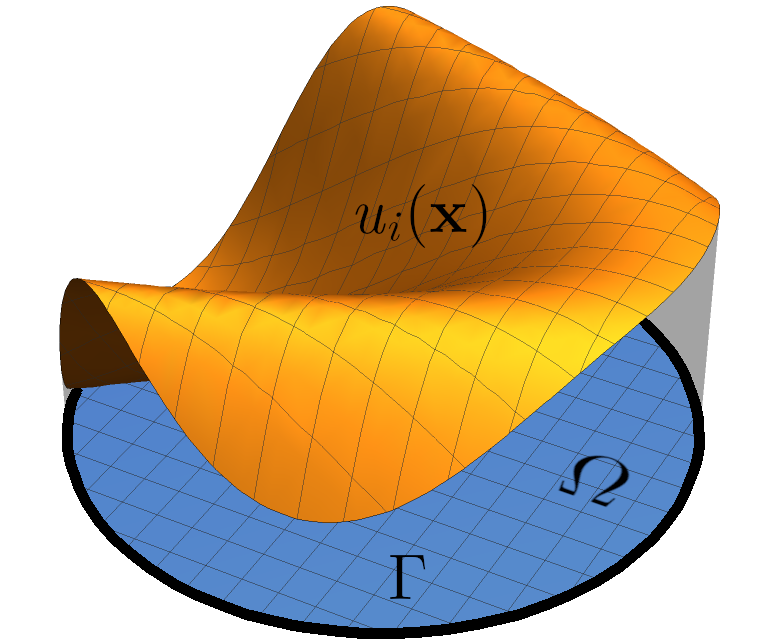
\includegraphics[width=5.5cm]{Slike/funkcijaInDomenaG}
	\caption{Domena $\Omega$, meja domene $\Gamma$ in komponenta rešitve $u_i(\mathbf{x})$.}
\label{fig:funkInDom}
\vspace{-2.6cm}
\end{wrapfigure}
Naj bo torej prizorišče dogajanja $d$-mnogoterost $\Omega$, opremljena s krajevnim vektorjem $\mathbf{x} = \{x_1, ..., x_d\}$. Pri reševanju sistema $m$ \texttt{PDE} iščemo nabor funkcij $\mathbf{u}(\mathbf{x}) =  \{u_1(\mathbf{x}), ..., u_m(\mathbf{x})\}$, ki v vsaki točki domene $\Omega$ zadosti sistemu \texttt{PDE}, na meji $\Gamma$ pa robnim pogojem (slika \ref{fig:funkInDom}). Konkretni primer bomo gradili na \textbf{sistemu Stokesovih enačb} za nestisljive tekočine v obliki \emph{u-p-$\omega$} (hitrost, tlak, vrtinčnost):\\[0.05cm]
\begin{minipage}{5.0cm}
\begin{IEEEeqnarray}{rl}
	\frac{\pd u}{\pd x} + \frac{\pd v}{\pd y} &= 0 \ , \label{eq:StokesDiv} \\[0.3cm]
	\alpha \frac{\pd p}{\pd x} + \beta \frac{\pd \omega}{\pd y} &= f_x \ ,
\end{IEEEeqnarray}
\end{minipage}
\begin{minipage}{5.3cm}
\begin{IEEEeqnarray}{rl}
	\gamma \frac{\pd p}{\pd y} - \delta \frac{\pd \omega}{\pd x} &= f_y \ , \\[0.3cm]
	\omega + \frac{\pd u}{\pd y} - \frac{\pd v}{\pd x} &= 0 \ , \label{eq:StokesCurl}
\end{IEEEeqnarray}
\end{minipage}\\[0.4cm]
ki jim za večjo nazornost primera umetno dodamo koeficiente $\alpha(\mathbf{x})$, $\beta(\mathbf{x})$, $\gamma(\mathbf{x})$ in $\delta(\mathbf{x})$ (v pravih enačbah jih ni). To je le sistem stacionarnih Navier-Stokesovih enačb brez nelinearnih konvektivnih členov, ki jih moramo pri numeričnem reševanju linearizirati. Ker ta korak za ponazoritev \texttt{LSFEM} ni ključen, se mu na tak način izognemo. Kot zanimivost navržimo, da Stokesove enačbe opisujejo plazeče se tokove, pri katerih je konvekcija gibalne količine (zaradi gibanja) majhna v primerjavi z njeno difuzijo (zaradi viskoznosti). V enačbah ni časovnih odvisnosti (razen preko časovno odvisnih robnih pogojev), zato so takšni tokovi časovno obrnljivi: časovno obrnjena rešitev enačb je prav tako rešitev (slika \ref{fig:TaylorCouette}).

\begin{figure}[!ht]
	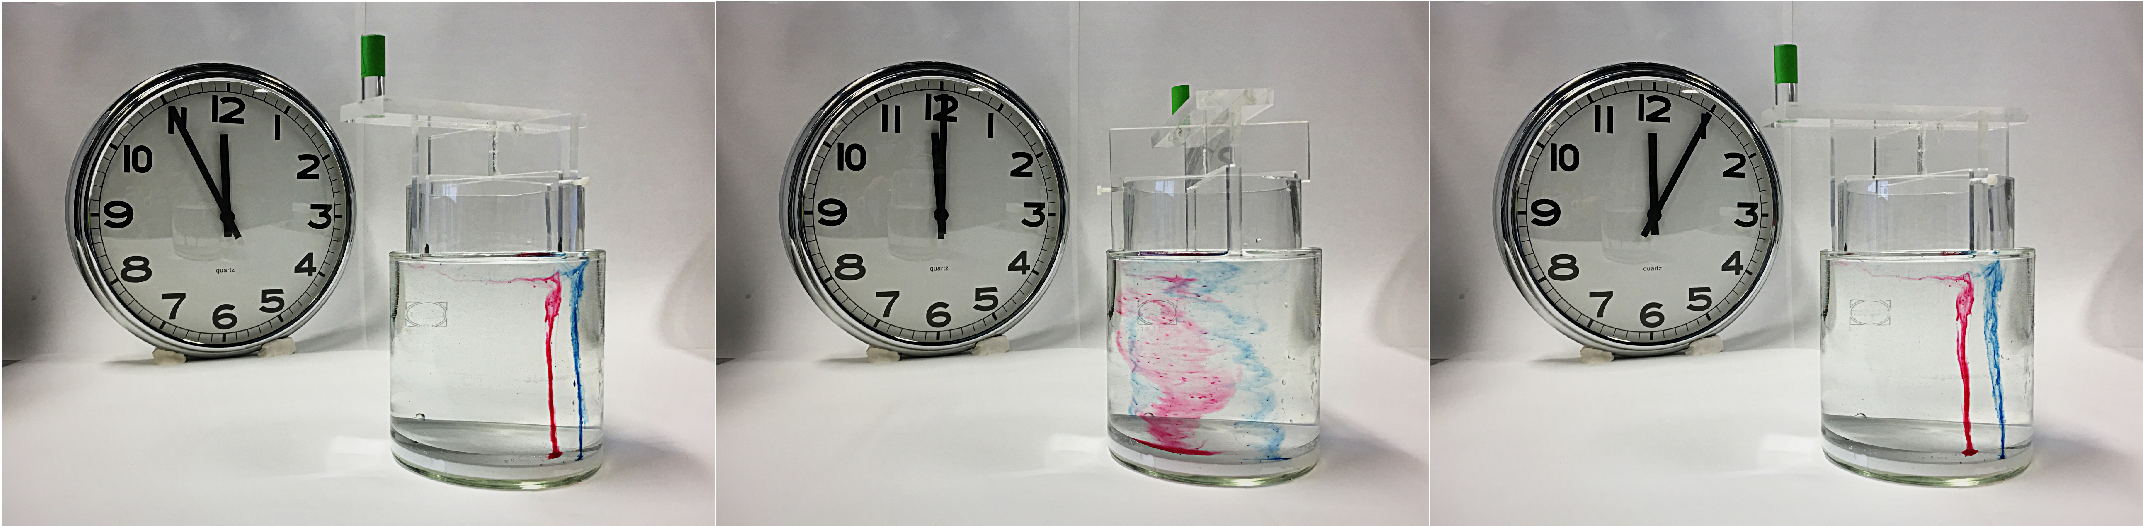
\includegraphics[width = 1\textwidth]{Slike/TaylorCouette}
	\caption{Zabaven eksperiment, pri katerem se v ozkem prostoru med dvema koncentričnima valjema nahaja viskozna tekočina, ki jo na dveh mestih označimo z liso barvila. Valja pet minut vrtimo v nasprotnih smereh (Stokesov tok, ki tako nastane, imenujemo Taylor-Couettov tok), da se lisi pomešata, nato smeri vrtenja obrnemo in po petih minutah se lisi ponovno sestavita. Pridobljeno iz  \cite{Wiki-StokesFlow}.}
	\label{fig:TaylorCouette}
	\vspace{-0.3cm}
\end{figure}

Sistem \texttt{PDE}, ki ga obravnavamo, zapišemo bolj jedrnato v matrični obliki. To je enostavno, če je sistem linearen. Uvedemo diferencialni operator $\mathbsf{A}$:
\begin{equation}
	\mathbsf{A}(\mathbf{x}) = \mathbsf{A}_0(\mathbf{x}) + \mathbsf{A}_1(\mathbf{x}) \frac{\pd}{\pd x_1} + \mathbsf{A}_2(\mathbf{x}) \frac{\pd}{\pd x_2} \ ,
\end{equation}

\setlength{\textheight}{26.4cm}
\pagebreak
\setlength{\topmargin}{1.6cm}			% Header Top Margin Height
\setlength{\headheight}{0.0cm}
\setlength{\headsep}{0.0cm}			% Header Lower Margin Height	 Footer height
\fancyhf{}
\fancyfoot[C]{\thepage}

s katerim lahko sistem enačb zapišemo kot:
\begin{IEEEeqnarray}{cc}
	\mathbsf{A}(\mathbf{x}) \cdot \mathbf{u}(\mathbf{x}) = \mathbf{f}(\mathbf{x}) \ . \label{eq:compactPDE} & \hspace{1.0cm} \texttt{jedrnat zapis PDE} \\[0.25cm]
	\left(\mathbsf{A}_0(\mathbf{x}) + \mathbsf{A}_1(\mathbf{x}) \frac{\pd}{\pd x_1} + \mathbsf{A}_2(\mathbf{x}) \frac{\pd}{\pd x_2}\right) \cdot \mathbf{u}(\mathbf{x}) = \mathbf{f}(\mathbf{x}) & \label{eq:matrixPDE1}
\end{IEEEeqnarray}
V matriko $\mathbsf{A}_0$ spravimo vse koeficiente pred členi z odvisnimi spremenljivkami, v matriko $\mathbsf{A}_1$ vse koeficiente pred členi z odvodi odvisnih spremenljivk po $x_1$ in v $\mathbsf{A}_2$ vse koeficiente pred členi z odvodi odvisnih spremenljivk po $x_2$. Ostale člene zložimo v vektor $\mathbf{f}$. Stokesove enačbe \eqref{eq:StokesDiv} - \eqref{eq:StokesCurl} lahko po zgledu enačbe \eqref{eq:matrixPDE1} zapišemo kot:
\begin{equation}
	\left[ \,
	\begin{pmatrix}
		0 & 0 & 0 & 0 \\
		0 & 0 & 0 & 0 \\
		0 & 0 & 0 & 0 \\
		0 & 0 & 0 & 1
	\end{pmatrix} +
	\begin{pmatrix}
		1 & 0 & 0 & 0 \\
		0 & 0 & \alpha & 0 \\
		0 & 0 & 0 & -\delta \\
		0 & -1 & 0 & 0
	\end{pmatrix} \frac{\pd}{\pd x} +
	\begin{pmatrix}
		0 & 1 & 0 & 0 \\
		0 & 0 & 0 & \gamma \\
		0 & 0 & \beta & 0 \\
		1 & 0 & 0 & 0 \\
	\end{pmatrix} \frac{\pd}{\pd y} \, \right]
	\ \cdot \
	\begin{pmatrix}
		u(\mathbf{x}) \\ v(\mathbf{x}) \\ p(\mathbf{x}) \\ \omega(\mathbf{x})
	\end{pmatrix}
	\ = \
	\begin{pmatrix}
		0 \\ f_x(\mathbf{x}) \\ f_y(\mathbf{x}) \\ 0
	\end{pmatrix} \ .
\end{equation}